\documentclass[border=10pt]{standalone}
\usepackage{tikz}
\usetikzlibrary{arrows.meta}
\tikzset{%
  >={Latex[width=2mm,length=2mm]},
  % Specifications for style of nodes:
            base/.style = {rectangle, rounded corners, draw=black,
                           minimum width=4cm, minimum height=1cm,
                           text centered, font=\sffamily},
  activityStarts/.style = {base, fill=blue!30},
       startstop/.style = {base, fill=red!30},
    activityRuns/.style = {base, fill=green!30},
         process/.style = {base, minimum width=2.5cm, fill=orange!15,
                           font=\ttfamily},
}
\begin{document}    
% Drawing part, node distance is 1.5 cm and every node
% is prefilled with white background
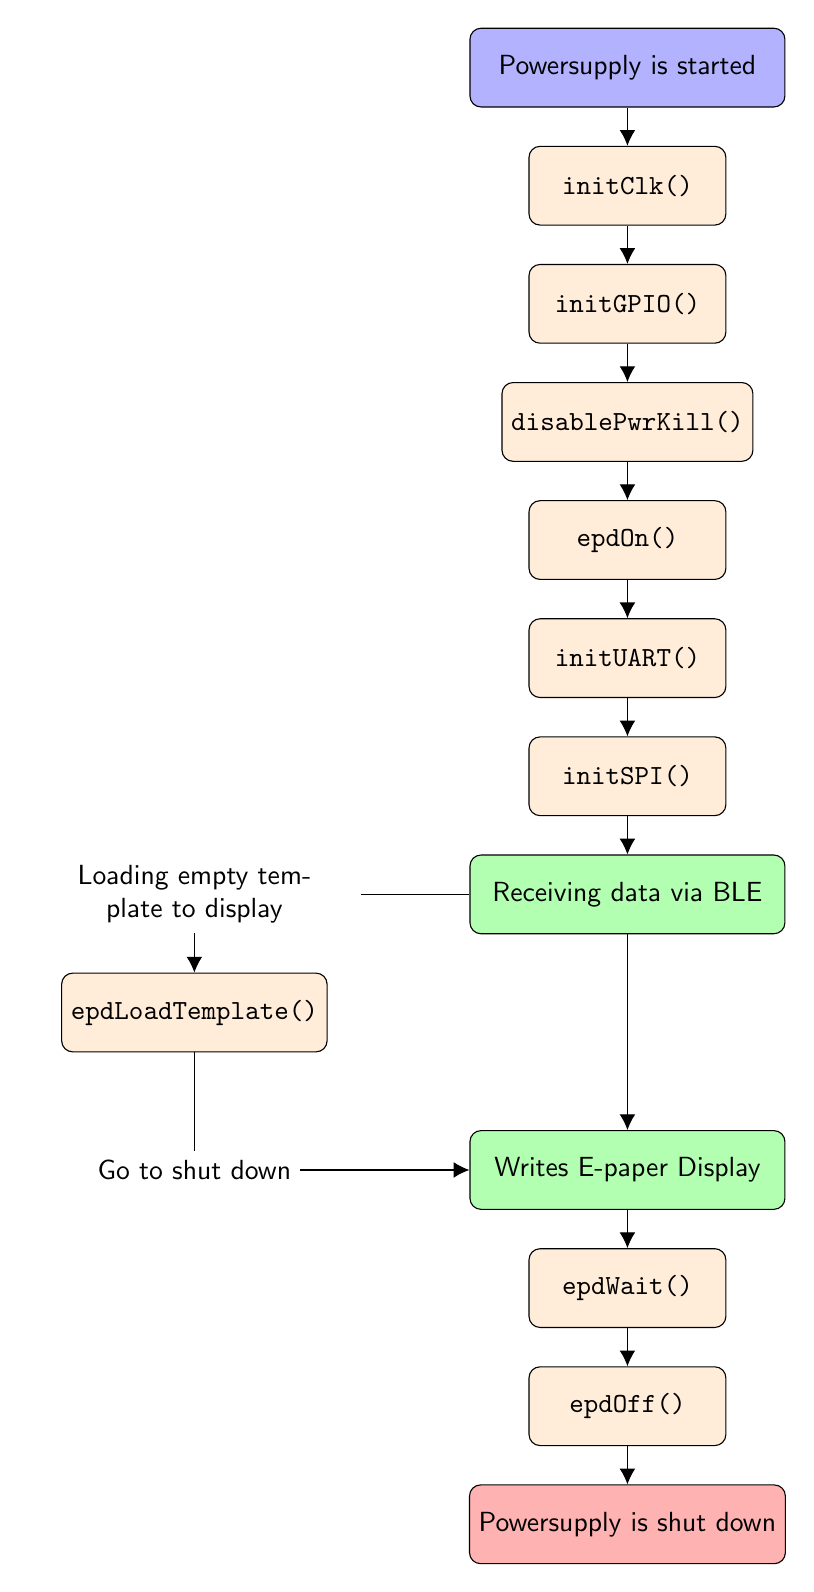
\begin{tikzpicture}[node distance=1.5cm,
    every node/.style={fill=white, font=\sffamily}, align=center]
    
  % Specification of nodes (position, etc.)
  \node (start)             [activityStarts]              {Powersupply is started};
  \node (initClock)     	[process, below of=start]          {initClk()};
  \node (initGPIO)      	[process, below of=initClock]   {initGPIO()};
  \node (disPwrKill)     	[process, below of=initGPIO]   {disablePwrKill()};
  \node (enPwrEPD)     		[process, below of=disPwrKill]   {epdOn()};
  \node (initUART)      	[process, below of=enPwrEPD] {initUART()};
  \node (initSPI)      		[process, below of=initUART] {initSPI()};
  
  \node (receiveData)      	[activityRuns, below of=initSPI] {Receiving data via BLE};
  \node (loadTemp)     		[process, left of=receiveData,xshift=-4cm,yshift=-1.5cm]   {epdLoadTemplate()};
  \node (writeEpd)      	[activityRuns, below of=receiveData,yshift=-2cm] {Writes E-paper Display};
  \node (Wait)      		[process, below of=writeEpd] {epdWait()};
  \node (offEpd)      		[process,below of= Wait] {epdOff()};

  \node (ActivityDestroyed) [startstop, below of=offEpd]
                                                    {Powersupply is shut down};     
  % Specification of lines between nodes specified above
  % with aditional nodes for description 
  \draw[->]             (start) -- (initClock);
  \draw[->]     	(initClock) -- (initGPIO);
  \draw[->]      	(initGPIO) 	-- (disPwrKill);
  \draw[->]     	(disPwrKill)-- (enPwrEPD);
  \draw[->]     	(enPwrEPD) 	-- (initUART);
  \draw[->]     	(initUART) 	-- (initSPI);
  \draw[->]     	(initSPI) 	-- (receiveData);
  \draw[->]     		(receiveData) 	-- (writeEpd);
  \draw[->]     	 (receiveData) -| node[text width=4cm]
                                   {Loading empty template to display} (loadTemp);
  \draw[->]      (loadTemp.south) |-node {Go to shut down}
                                   (writeEpd);
  \draw[->]       (writeEpd) --  (Wait);
  \draw[->]    (Wait) -- (offEpd);
  \draw[->]       (offEpd) --        (ActivityDestroyed);
 
  \end{tikzpicture}
\end{document}